%
% File acl2015.tex
%
% Contact: car@ir.hit.edu.cn, gdzhou@suda.edu.cn
%%
%% Based on the style files for ACL-2014, which were, in turn,
%% Based on the style files for ACL-2013, which were, in turn,
%% Based on the style files for ACL-2012, which were, in turn,
%% based on the style files for ACL-2011, which were, in turn, 
%% based on the style files for ACL-2010, which were, in turn, 
%% based on the style files for ACL-IJCNLP-2009, which were, in turn,
%% based on the style files for EACL-2009 and IJCNLP-2008...

%% Based on the style files for EACL 2006 by 
%%e.agirre@ehu.es or Sergi.Balari@uab.es
%% and that of ACL 08 by Joakim Nivre and Noah Smith

\documentclass[11pt]{article}
\usepackage{acl2015}
\usepackage{times}
\usepackage{url}
\usepackage{latexsym}
\usepackage{amsopn}

%%%%%%%%%%%%%%%%%%%%%%%%%%%%%%%%%%%%%%%%%%%%%%%%%%%%%%%%%%%%%%%%%%%%
%% KUI'S STANDARD PREAMBLE
%%%%%%%%%%%%%%%%%%%%%%%%%%%%%%%%%%%%%%%%%%%%%%%%%%%%%%%%%%%%%%%%%%%%

\usepackage{subfigure}
\usepackage{algorithm}
\usepackage{algorithmicx}
\usepackage{algpseudocode}
\usepackage{xcolor}
\usepackage{tabularx}

\usepackage{graphicx}
\DeclareMathOperator{\conv}{conv}
\DeclareMathOperator{\st}{s.t.}
\DeclareMathOperator{\dom}{dom}
\DeclareMathOperator{\im}{im}
\DeclareMathOperator{\Ne}{Ne}
\DeclareMathOperator{\sign}{sign}
\DeclareMathOperator{\Var}{Var}
\DeclareMathOperator{\diag}{diag}
\DeclareMathOperator{\vvec}{vec}


%\setlength\titlebox{5cm}

% You can expand the titlebox if you need extra space
% to show all the authors. Please do not make the titlebox
% smaller than 5cm (the original size); we will check this
% in the camera-ready version and ask you to change it back.

\title{Topic Models for Texts and Images in Representation Space}

\author{Kui Tang \\
  Columbia University \\
  {\tt kt2384@columbia.edu} \\\And
  Sameer Lal \\
  Columbia University \\
  {\tt sl3368@columbia.edu} \\}
%\date{10 May 2015}
\date{}

\begin{document}
\maketitle
\begin{abstract}
The abstract goes here.
\end{abstract}

\section{Introduction}
One of the popular tasks in Machine Learning and Computer Vision has been object detection. The ability for computers to recognize patterns in image data has many applications in robotics, health care, manufacturing, and defense. For many years, traditional computer vision algorithms were capable of achieving mediocre performance in object recogntion challenges. Recently though, the use of convolutional neural networks has led researchers to achieve significantly higher levels of performance. This breakthrough has been met with a rapid adoption of deep learning in many other domains. Neural nets have been used in natural language processing, speech recognition, facial detection, and reinforcement learning. Having developed a powerful tool for supervised learning across multiple modalities of data, a new challenge arises in performing learning in this multimodal space. Given the ability to extract rich features via neural networks and the abundance of unsupervised multimodal data, research focus has shifted to building models which could learn semantic information from these natural data sets such as news articles or annotated images. By extracting features from this space, statistical models could gain a much deeper understanding of objects and concepts. 

\section{Related Work}
\paragraph{Neural multimodal models.}
\cite{Lecun98} propose joining several neural network models for multimodal learning into a joint objective function, and then optimizing the parameters of each to maximize performance on this joint measure. \cite{Srivastava14} propose a joint text-image model using RBMs. Their model is fully generative, and the textual model is an undirected analogue to a topic model. However, they are unable to leverage state-of-the-art CNN image features, and they rely on contrastive divergence for learning, which limits scalability. They also rely on a binary semantic space, while ours is real.

\paragraph{Topic models on shallow image features.}
Several authors have applied topic modeling to visual or joint text and visual data, but none to date have utilized deep semantic representations as image features. \cite{Barnard03} considers several models beginning with marginally independent emission distributions for words and image blobs (which are nevertheless conditional dependent) and proceeds to model additional dependencies between the distributions. \cite{Wang09} model alignment between words and image patches, but train on a supervised dataset and use only bag of codeword features to represent images, with codewords generated by $k$-means and SIFT. Moreover, these methods are designed only for supervised image captioning.

Some work has used topic models in unsupervised settings for images. \cite{Fritz08} trains LDA to detect object categories, but they use only gradient histogram representations. \cite{Cao07} proposed a model for unsupervised object detection, but they only used quantized SIFT features.

\paragraph{Hybrid neural network and HMM models.}
A simpler problem related to our work is to combine output from a feedforward neural network with a Hidden Markov model. Several authors have proposed schemes tuned for a variety of tasks \cite{Trentin01}. The approach closest to ours is that of \cite{Bengio92}, which derives gradient updates to a feedforward neural network based on the maximum-likelihood objective. Our work shares the same approach to optimize the neural network parameters to maximize the likelihood of the overall probabilistic model.

\section{Models}
\begin{figure}
\centering
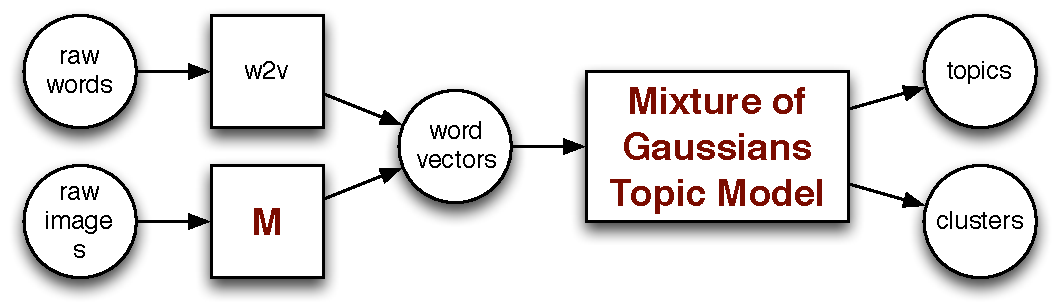
\includegraphics[width=\columnwidth]{assets/stagewise_model.pdf}
\caption{Diagram of stagewise multimodal model of this work. Black boxes denote standard pretrained models. Round entries are intermediate representations, and green boxes denote components we trained.}
\end{figure}
\subsection{Mapping Image Vectors to Word Vectors}

\subsection{Gaussian Topic Model}
The model assumes a large dictionary of ``concepts'', which are Gaussian clusters in semantic space. A topic is a mixture of these concepts, and each vector $x_{dn}$ (word or image) is described by a mixture of topics. The generative process is as follows:
\begin{itemize}
\item For $k = 1, \ldots, K$ (for each topic):
  \begin{itemize}
    \item Draw $\beta_k \sim \mbox{Dir}(\alpha)$
    \item Draw $\lambda_k \sim \mbox{Gamma}(10^{-6}, 10^{-6})$
    \item Draw $\mu_k \sim \mathcal{N}(0, \diag(\tau))$
  \end{itemize}
\item For $d = 1, \ldots, D$ (for each document):
  \item Draw $\theta_d \sim \mbox{Dir}(\gamma)$
  \item For $n = 1, \ldots, N_d$ (for each word in document):
  \begin{itemize}
    \item Draw $z_{dn} \sim \mbox{Mult}(\theta_{dn})$
    \item Draw $c_{dn} \sim \mbox{Mult}(\beta_{z_{dn}})$
    \item Draw $x_{dn} \sim \mathcal{N}(\mu_{c_{dn}}, \diag(\tau_{c_{dn}})$
  \end{itemize}
\end{itemize}

\section{Results}

\subsection{Data}
\label{sec:data}
Image vector data was extracted using the popular image processing library Caffe (SHOULD CITE). The library's pretrained CaffeNet convolutional neural net was 

\subsection{Image-Word Alignment Results}

\subsection{Mixture of Gaussian Topic Model Results}

\begin{figure}
\centering
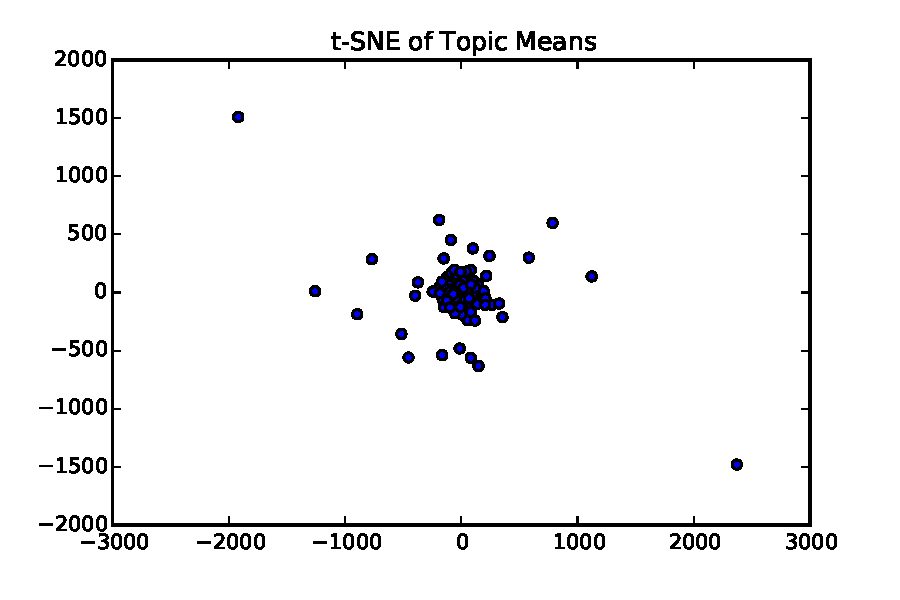
\includegraphics[width=\columnwidth]{assets/gtm100_mu_tsne.pdf}
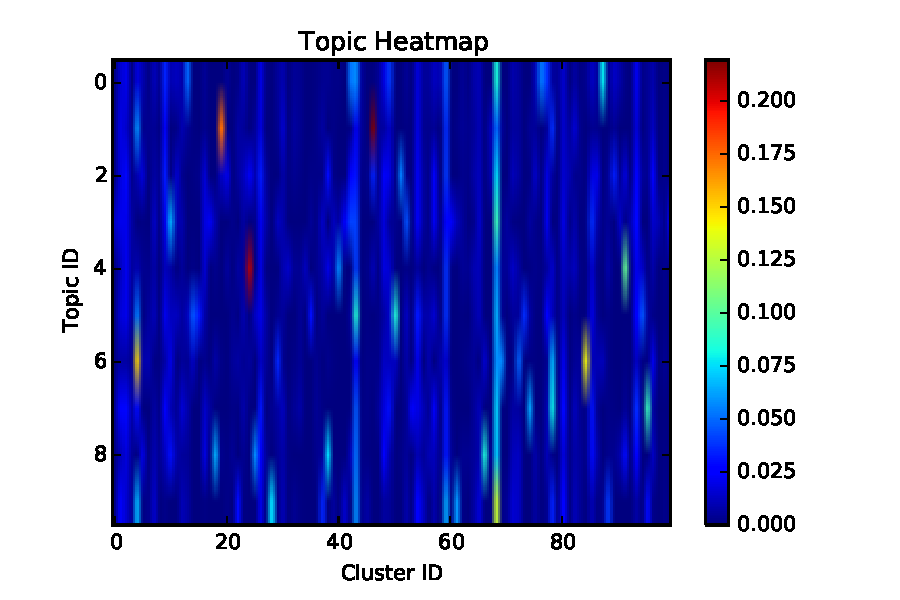
\includegraphics[width=\columnwidth]{assets/gtm100_topic_heatmap.pdf}
\caption{\emph{Top:} Locations of means of 100 concept clusters ($t$-SNE). \emph{Bottom:} Distribution of topics (rows) over clusters (columns).}
\end{figure}

\begin{figure}
\centering
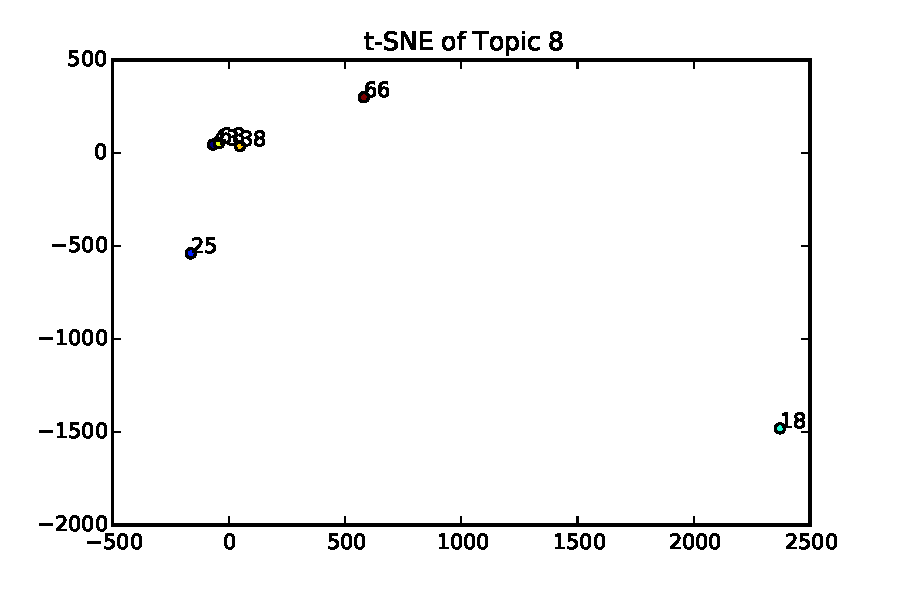
\includegraphics[width=\columnwidth]{assets/gtm100_topic8_tsne.pdf}
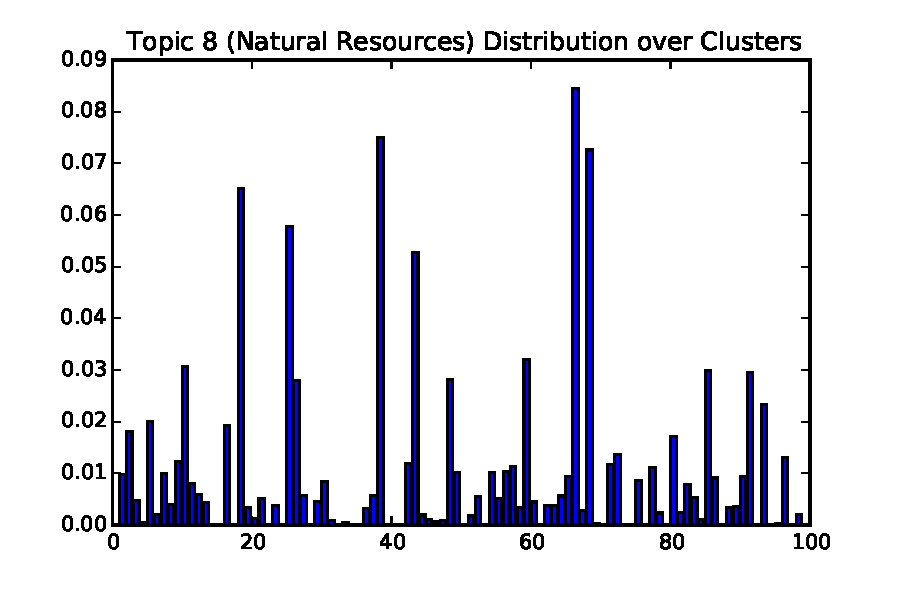
\includegraphics[width=\columnwidth]{assets/gtm100_topic8_probs.pdf}

\begin{tabularx}{\columnwidth}{|c|X|}
\hline 
{\tiny{}Cluster} & {\tiny{}Words}\tabularnewline
\hline 
{\tiny{}18} & {\tiny{}\textbf{[Saltwater]} shoreline ocean coastline nearshore\_reefs sandy\_shorelines
coastal\_waters shallow\_reefs tidal\_creek shallow\_waters mud\_flats
sea tidal\_inlet pier\_pilings underwater reef shoreward abyssal\_plain
inter\_tidal shifting\_sandbars sandy\_bottomed }\tabularnewline
\hline 
{\tiny{}25} & {\tiny{}\textbf{[Freshwater]} water ice surface green porpoise\_vaults surficial\_aquifer
rainwater Floridan\_aquifer radar\_deflectors wa\_ter absorbs\_carbon\_dioxide
bermed absorbs\_sunlight bugs\_wiggling Mosquitoes\_breed overflowing\_septic\_tanks
mild\_dishwashing\_liquid reverse\_osmosis\_filtration hyper\_saline
secondary\_clarifier }\tabularnewline
\hline 
{\tiny{}38} & {\tiny{}\textbf{[Chemicals]} hydrous calcium\_oxide cyclohexane inorganic\_salts calcium\_sulphate
fluorocarbons Sodium\_cyanide silicate\_rocks Nitric\_acid chemically\_reactive
calcium\_carbonates magnesium\_silicate outgas raffinate potassium\_salts
bacterial\_decomposition methane trihalomethanes\_THMs element\_boron
Sulphur\_dioxide }\tabularnewline
\hline 
{\tiny{}66} & {\tiny{}\textbf{[Volcanoes]} coral reefs reef corals coral\_reefs ocean volcanoes sea coral\_reef
volcanic islands lava volcano oceans undersea\_volcanoes oceanic ocean\_basins
lava\_flows eruptions Kilauea\_Volcano}\tabularnewline
\hline 
\end{tabularx}

\caption{\emph{Top:} Locations of means of significant ($\geq 5\%$ posterior probability) concept clusters for the ``natural resources'' topic ($t$-SNE). \emph{Bottom:} Distribution over concept clusters for the ``Natural resources'' topic.}
\end{figure}

\begin{table}
\centering
\begin{tabular}{|c|c|c|}
\cline{2-3} 
\multicolumn{1}{c|}{} & LDA & MoG-LDA\tabularnewline
\hline 
Test log-likelihood & -11.915 & \tabularnewline
\hline 
Test perplexity & 3860.5 & \tabularnewline
\hline 
Avg. observed coherence & 0.00509 & 0.01666 \tabularnewline
\hline 
Avg. word intrusion & 0.60 & 0.30 \tabularnewline
\hline 
\end{tabular}
\caption{Quantitative results comparing mixture of Gaussian topic model (with pretrained word vectors) with ordinary LDA. All log-likelihood and perplexity results were obtained by training on last 100 documents and testing on first 100 as described in Sec.~\ref{sec:data}. The topic coherence metrics are described in \cite{Lau14} using code supplied by the author.}
\end{table}

\section{Discussion}

\section{Conclusions and Future Work}

\section*{Acknowledgments}

We thank Profs. Liangliang Cao and James Fan for organizing a deep learning course, encouraging us to explore multimodal models, and for their advice on evaluation.

% include your own bib file like this:
\bibliographystyle{acl}
\bibliography{ML}

%\begin{thebibliography}{}
%\end{thebibliography}

\end{document}
